\documentclass{article}
\usepackage[utf8]{inputenc}
\usepackage{graphicx}


\title{Cara Menambahkan aplikasi di apex oracle}
\author{yukiardiansyah321 }
\date{October 2019}

\begin{document}

\maketitle

\section{Pembuatan Aplikasi}

\begin{enumerate}
    \item langkah pertama dalam pembuatan aplikasi baru di apex online melalui excel adalah dengan membuat sebuah data yang akan kita masukan dalam apex oracle online. data yang akan di masukkan sesuai data yang telah di buat contoh saya memasukkan data Perkuliahan dan menambahkan 5 buah table yaitu mahasiswa
    ,dosen,kuliah,jadwal,nilai
    \begin{center}
         \centering
            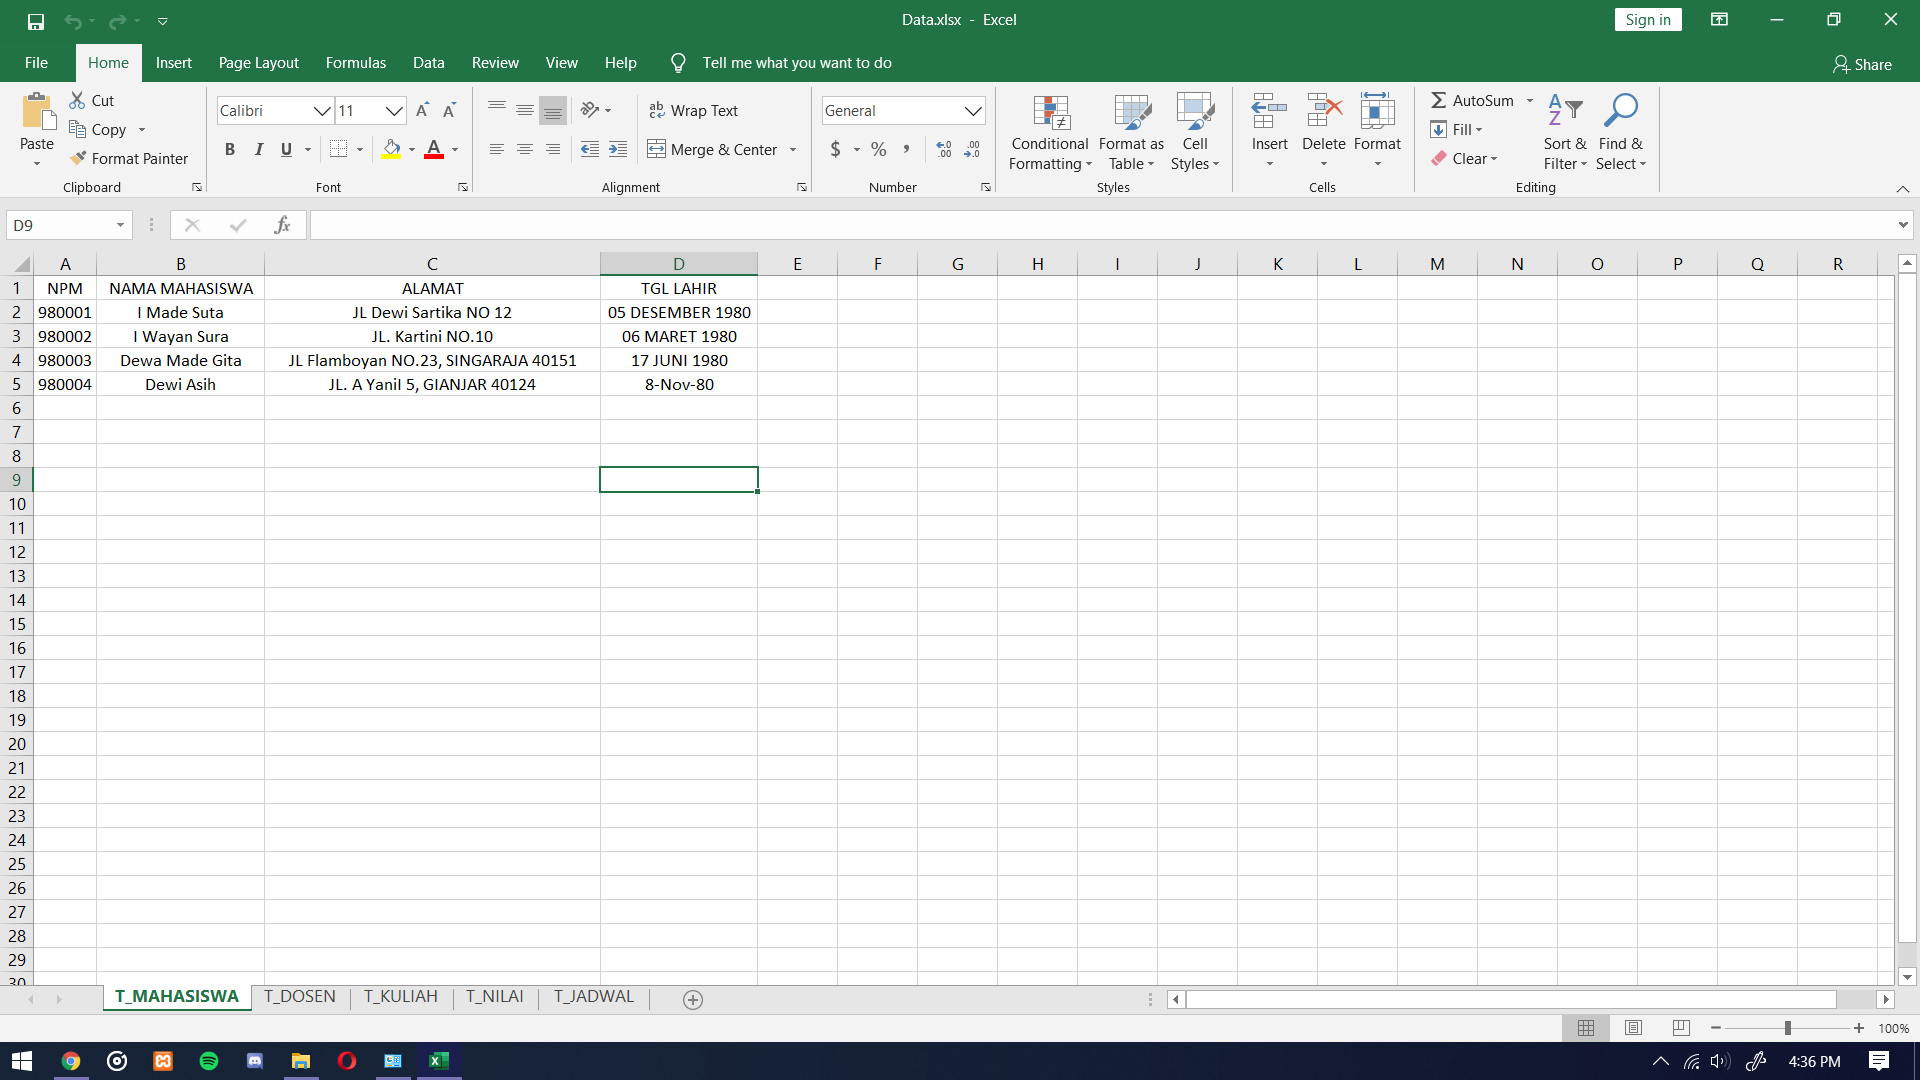
\includegraphics[scale=0.27]{figures/DB0.png}
        \caption{Menambahkan Data Di Excel}
        \label{excel}
    \end{center}
       
     \item langkah selanjutnya buka di browser apex oracle online setelah itu klik ap builder dan create  
    \begin{center}
         \centering
            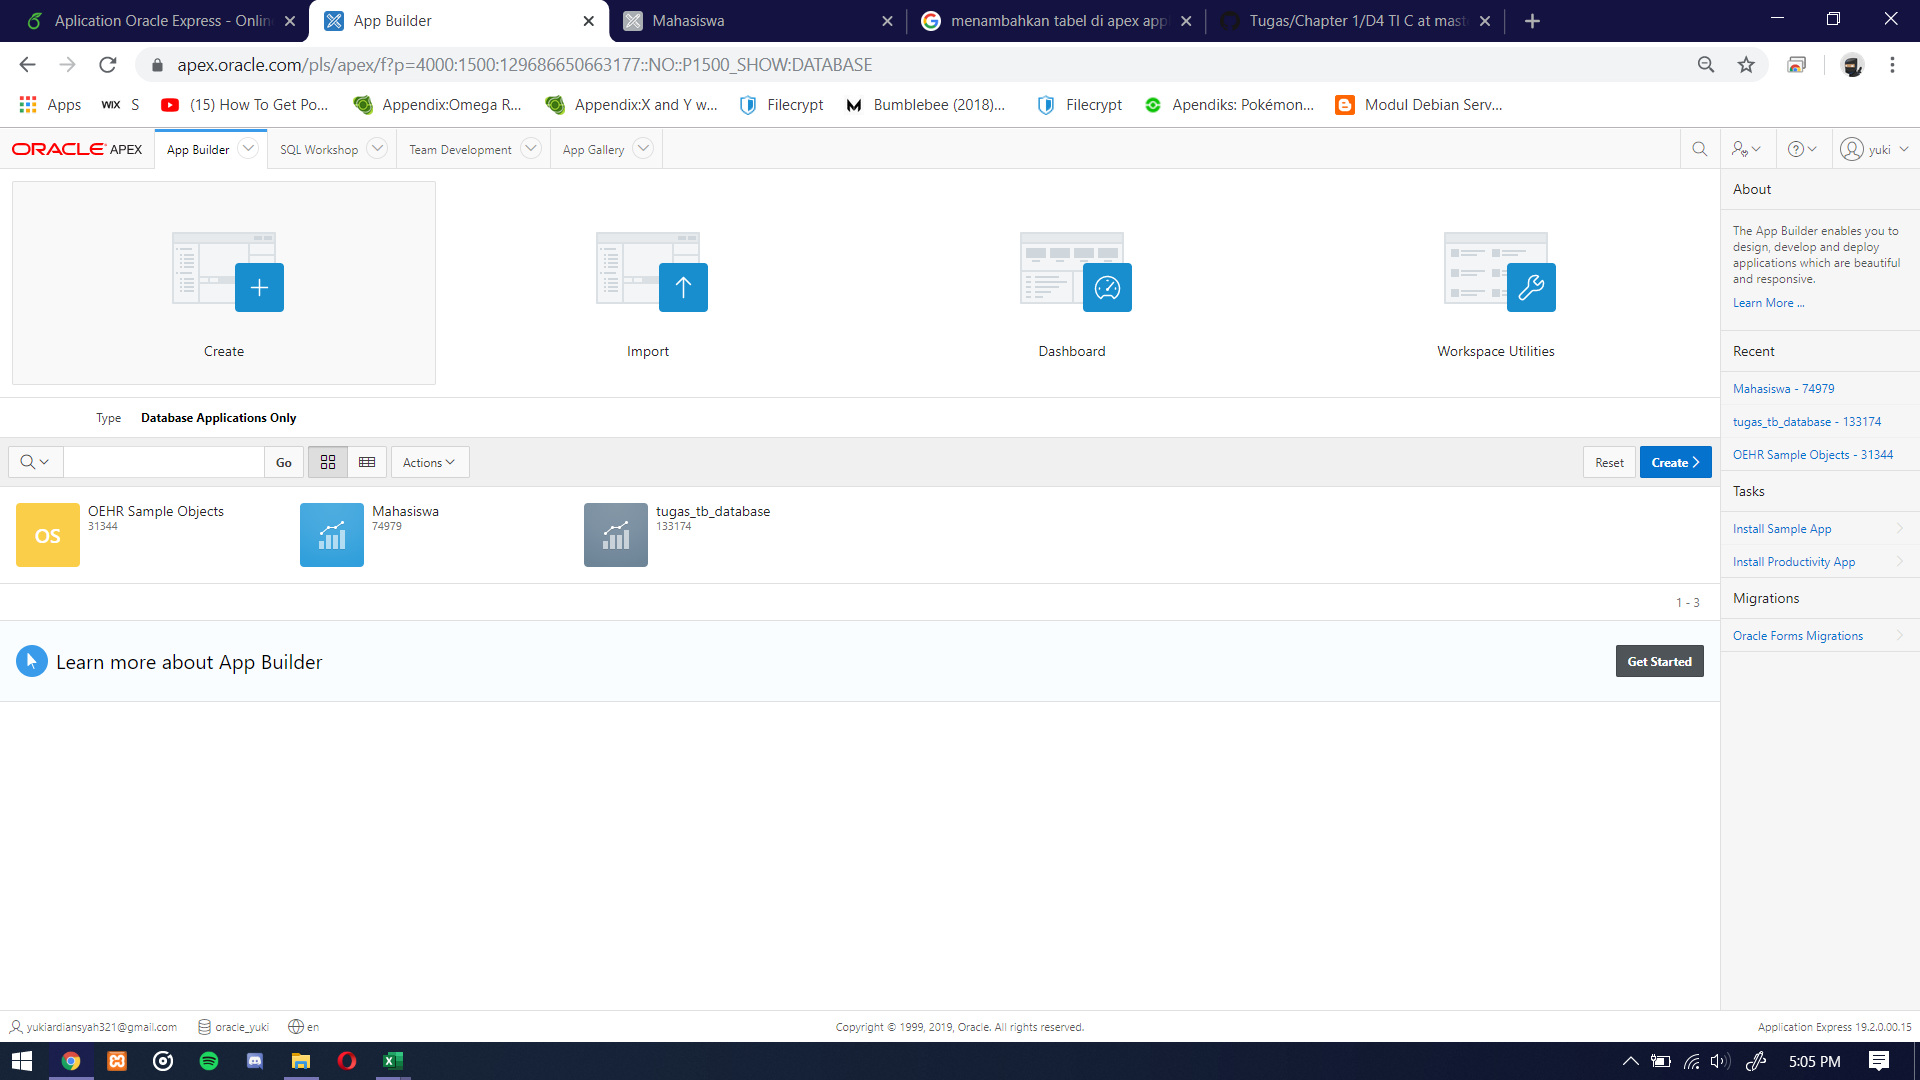
\includegraphics[scale=0.27]{figures/DB1.png}
        \caption{Buka Apex Oraacle }
        \label{create}
    \end{center}
    
      \item Setelah mengklik create kita melihat 3 cara menambahkan data dalam aplikasi yang ingin di buat klik from a file agar dapat memilih file excel yang telah dibuat
    \begin{center}
         \centering
            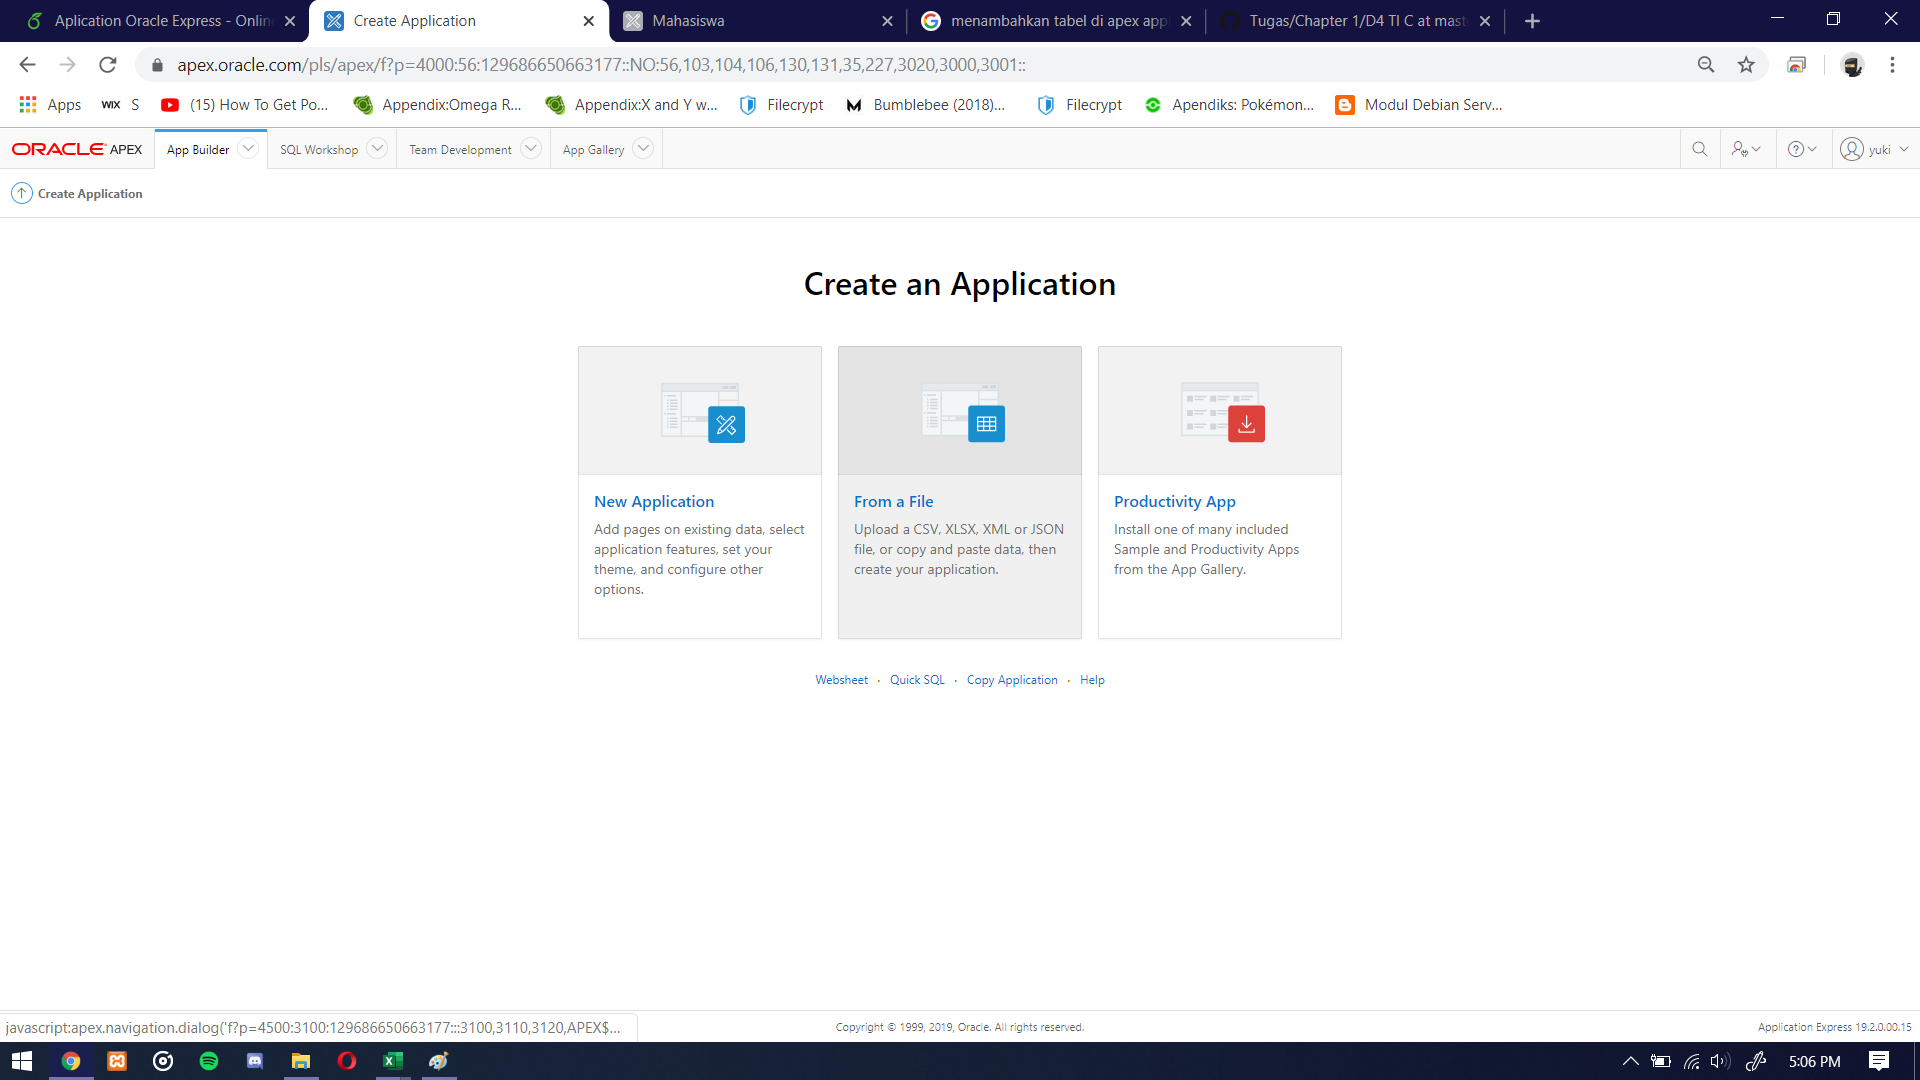
\includegraphics[scale=0.27]{figures/DB2.png}
        \caption{chosse a file}
        \label{from}
    \end{center}
    
    \item Setelah mengklik pilihan from a file system akan menampilkan load data yang berguna untuk memilih jenis file apa yang akan direlafikasi menjadi sebuah table. klik chosse file from a computer untuk memilih file excel yang telah di buat
    \begin{center}
         \centering
            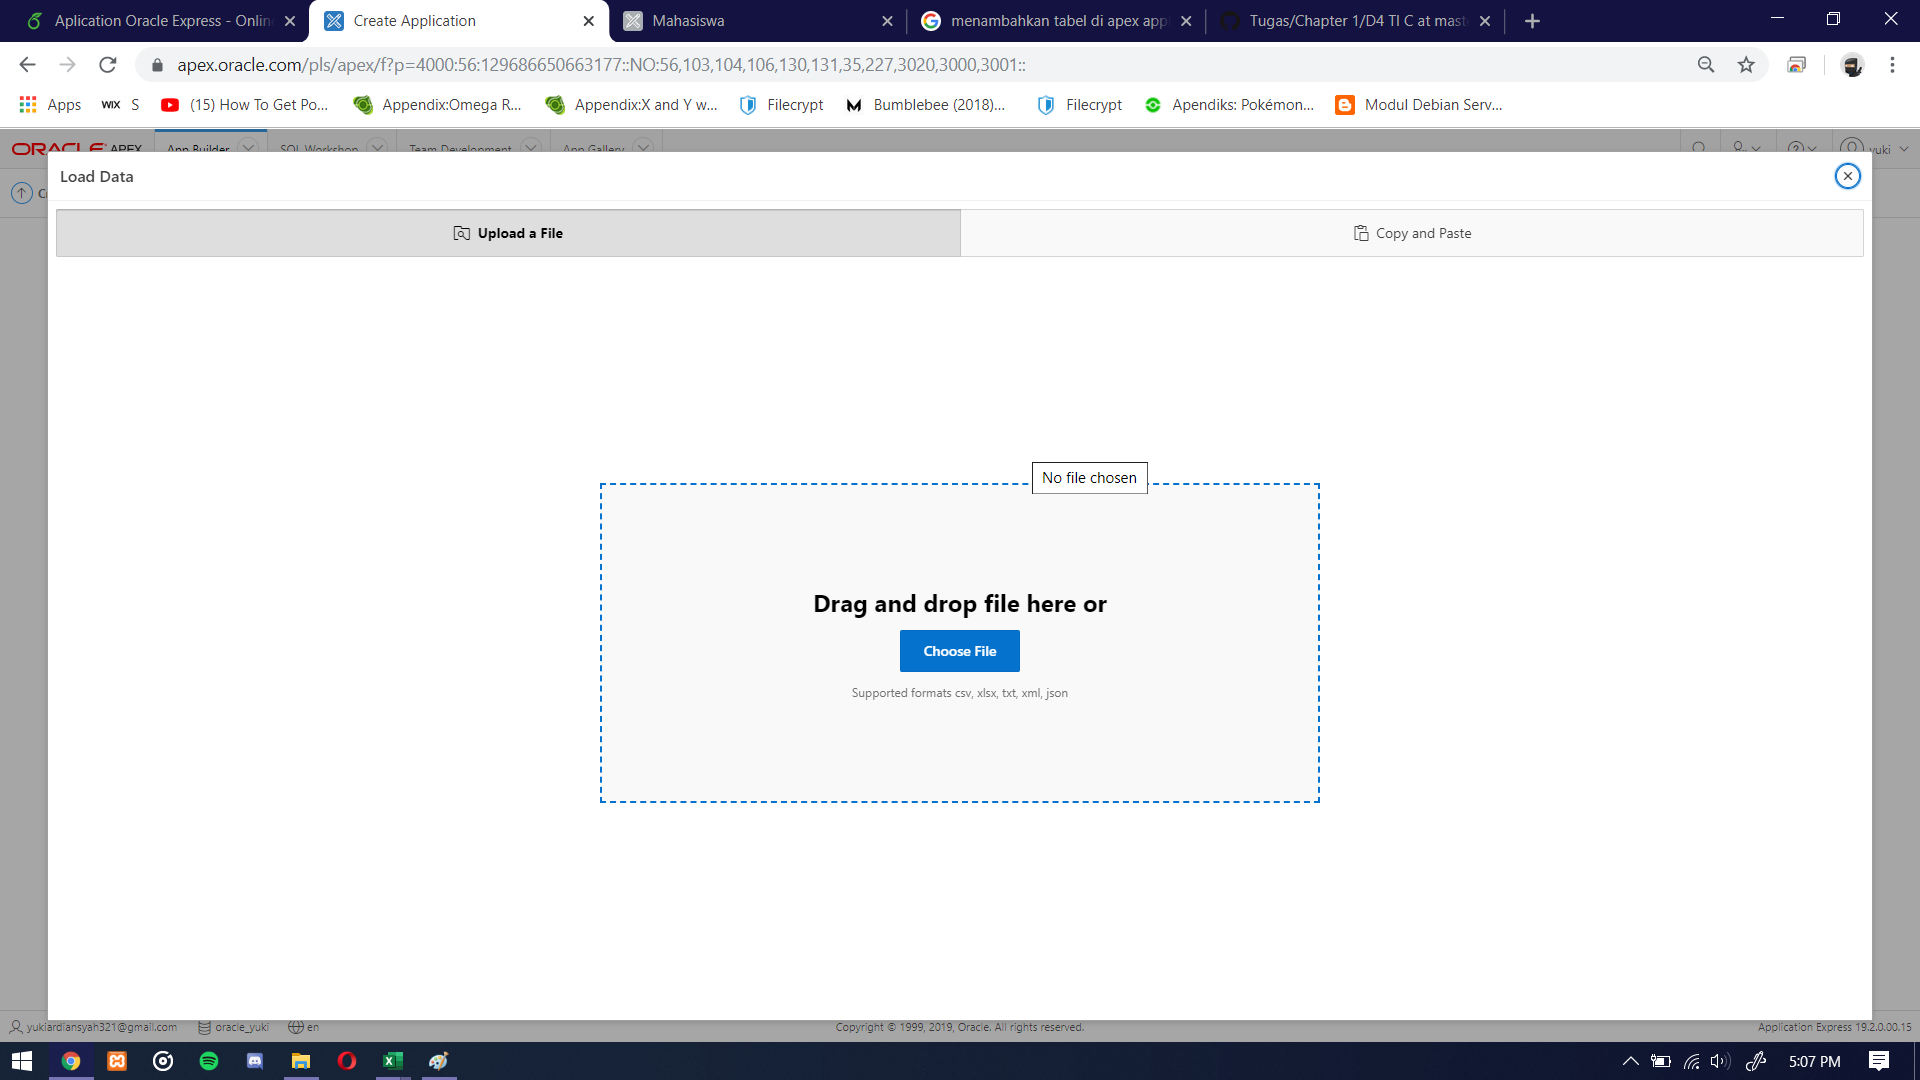
\includegraphics[scale=0.27]{figures/DB3.png}
        \caption{LOAD DATA}
        \label{chosse}
    \end{center}
    
     \item Setelah mendrag file excel tersebut kemudian memilih select sheet dari data mahasiswa agar table yang akan dibuat keluar data mahasiswa. lakukan hal yang sama pada ke 5 data table tersebut seperti dosen,kuliah,jadwal dan nilai
    \begin{center}
         \centering
            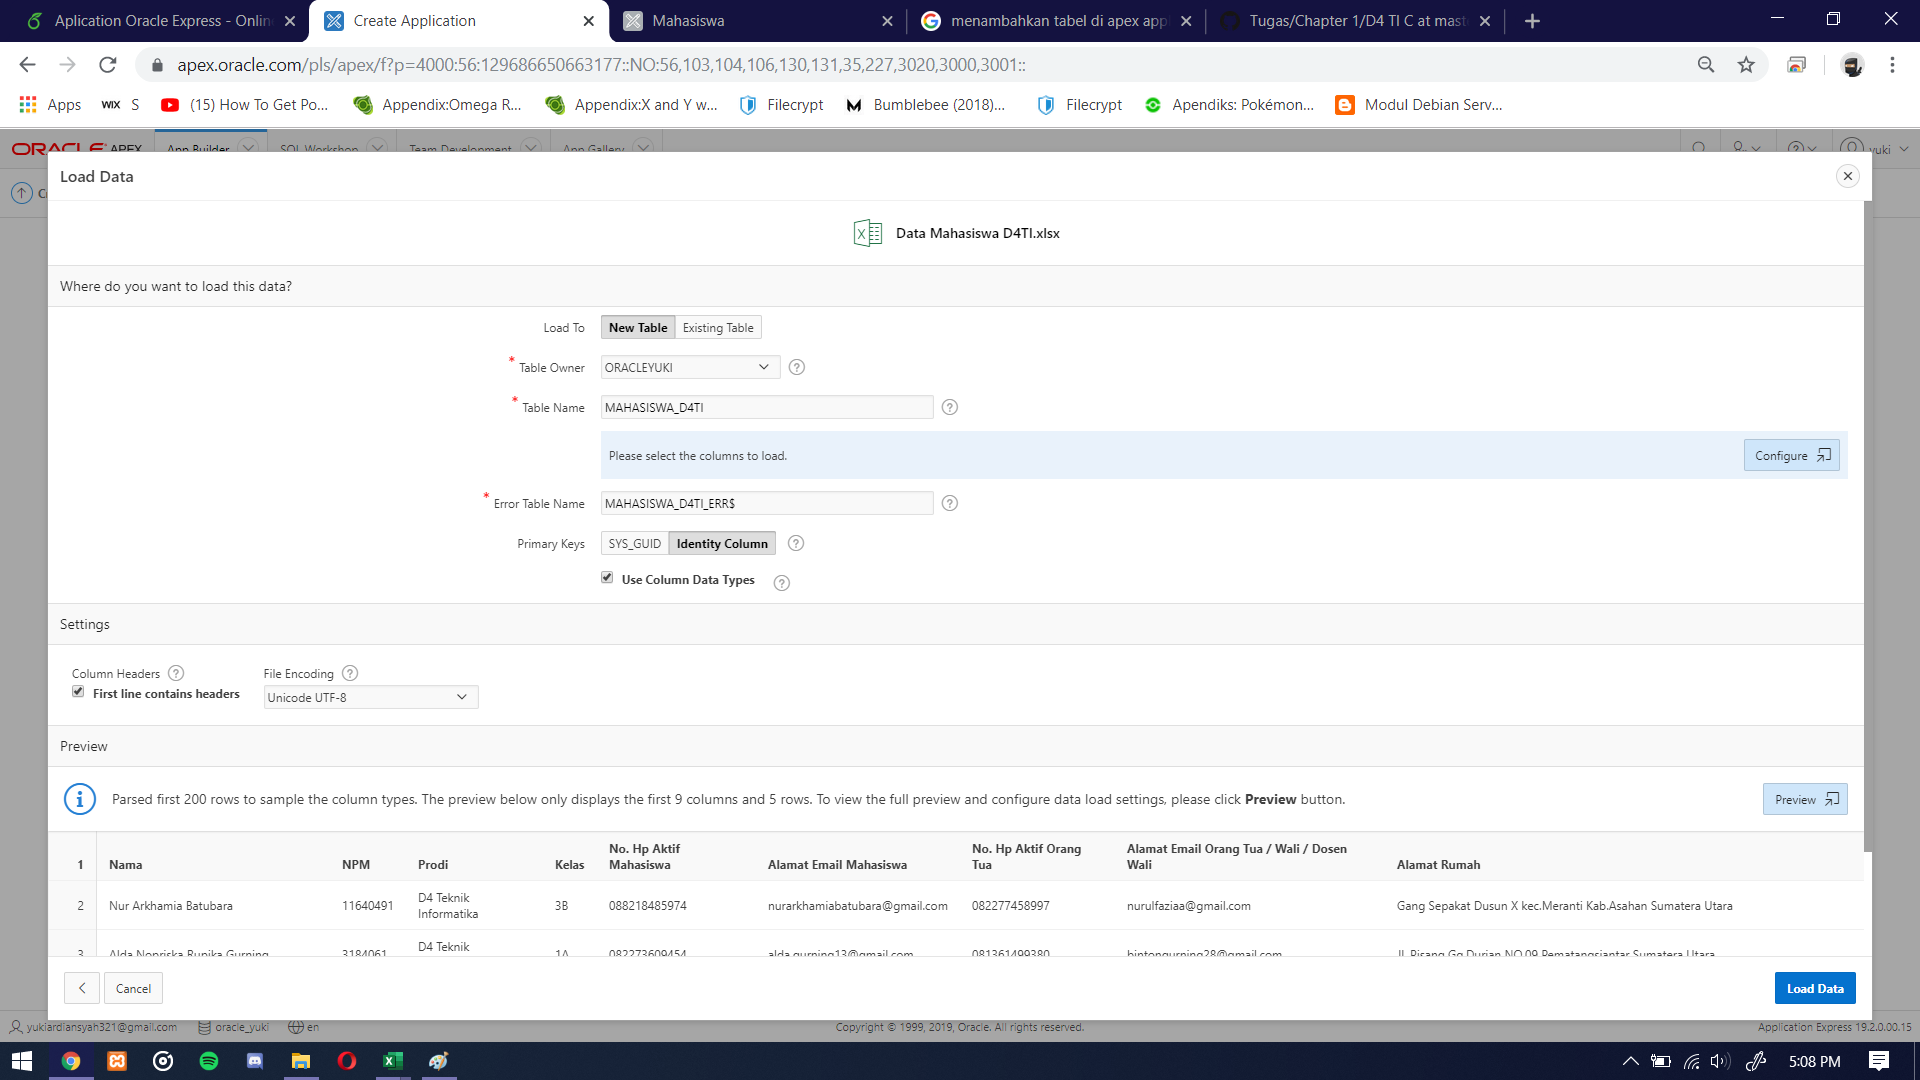
\includegraphics[scale=0.27]{figures/DB4.png}
        \caption{Menamai Table }
        \label{excel}
    \end{center}
    
     \item Setelah kelima table di tamabahkan ke dalam apex oracle cek apakah datanya sudah masuk atau belum di dalam object browser
      \ref{excel}
    \begin{center}
         \centering
            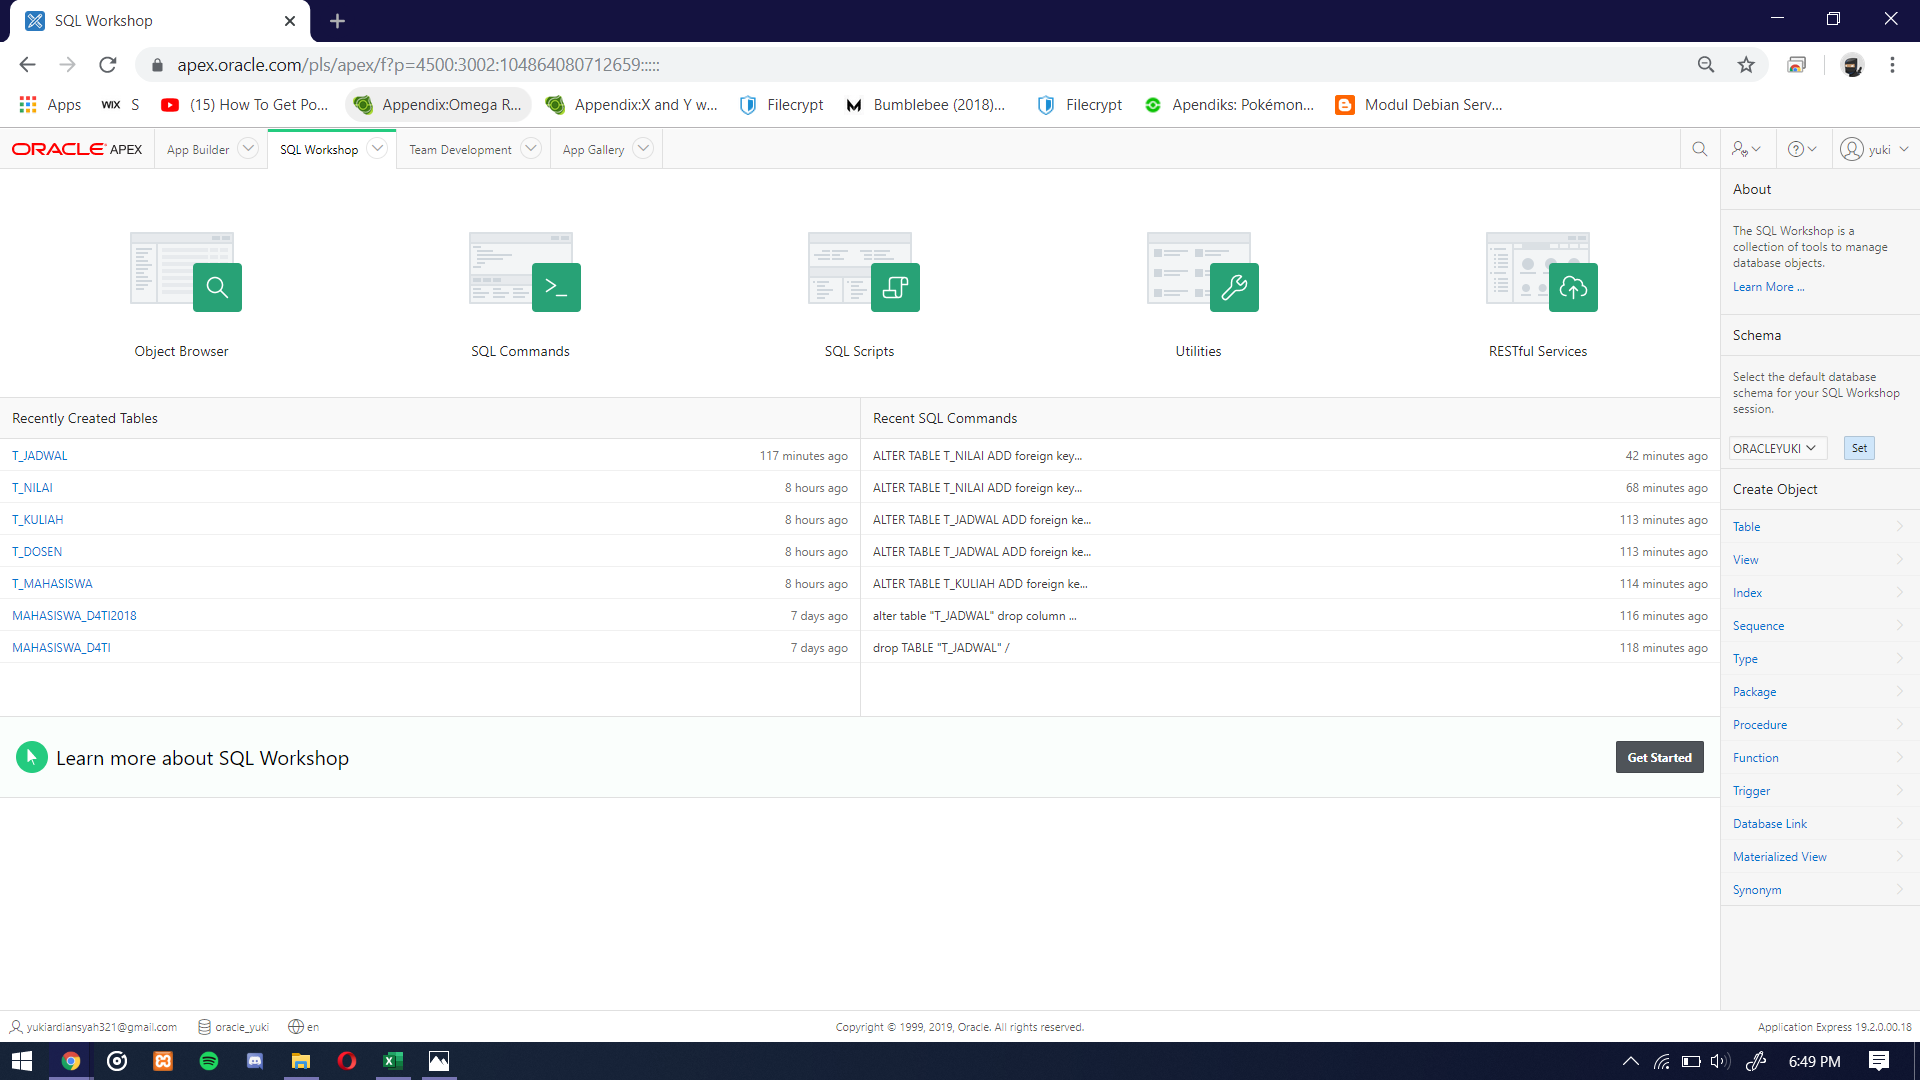
\includegraphics[scale=0.27]{figures/DB5.png}
        \caption{Melihat Table Yang Sudah}
        \label{excel}
    \end{center}
    
     \item Setelah kelima table tersimpan kita akan membuat primary key di table mahasiswa,dosen dan kuliah dengan kodingan seperti yang ada di gambar dibawah ini
    \begin{center}
         \centering
            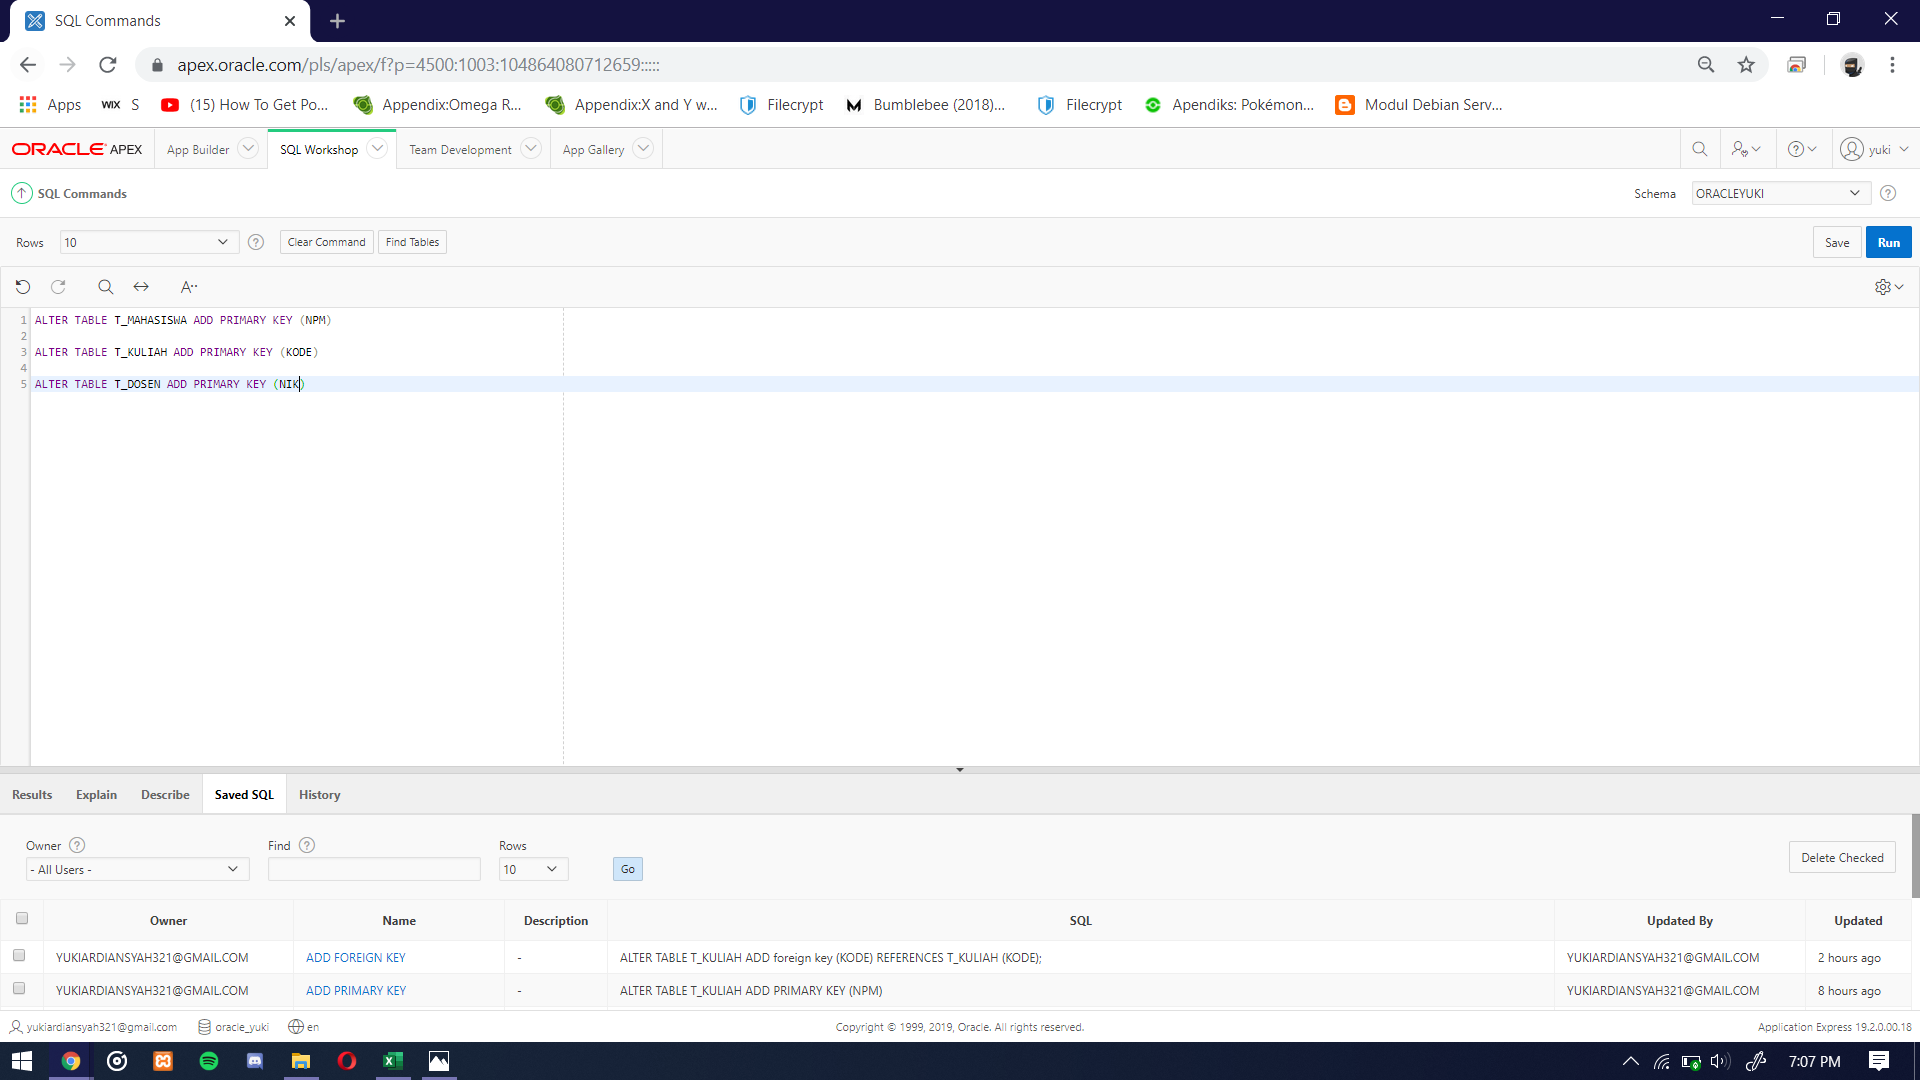
\includegraphics[scale=0.27]{figures/DB6.png}
        \caption{Membuat Primary Key}
        \label{excel}
    \end{center}
    
      \item Setelah ketiga table ditambahkan primary key langkah selanjutnya adalah melakukan relasi dengan mengetikan kodingan untuk menambahkan foreign key di table jadwal dan nilai sesuai dengan gambar di bawah ini 
    \begin{center}
         \centering
            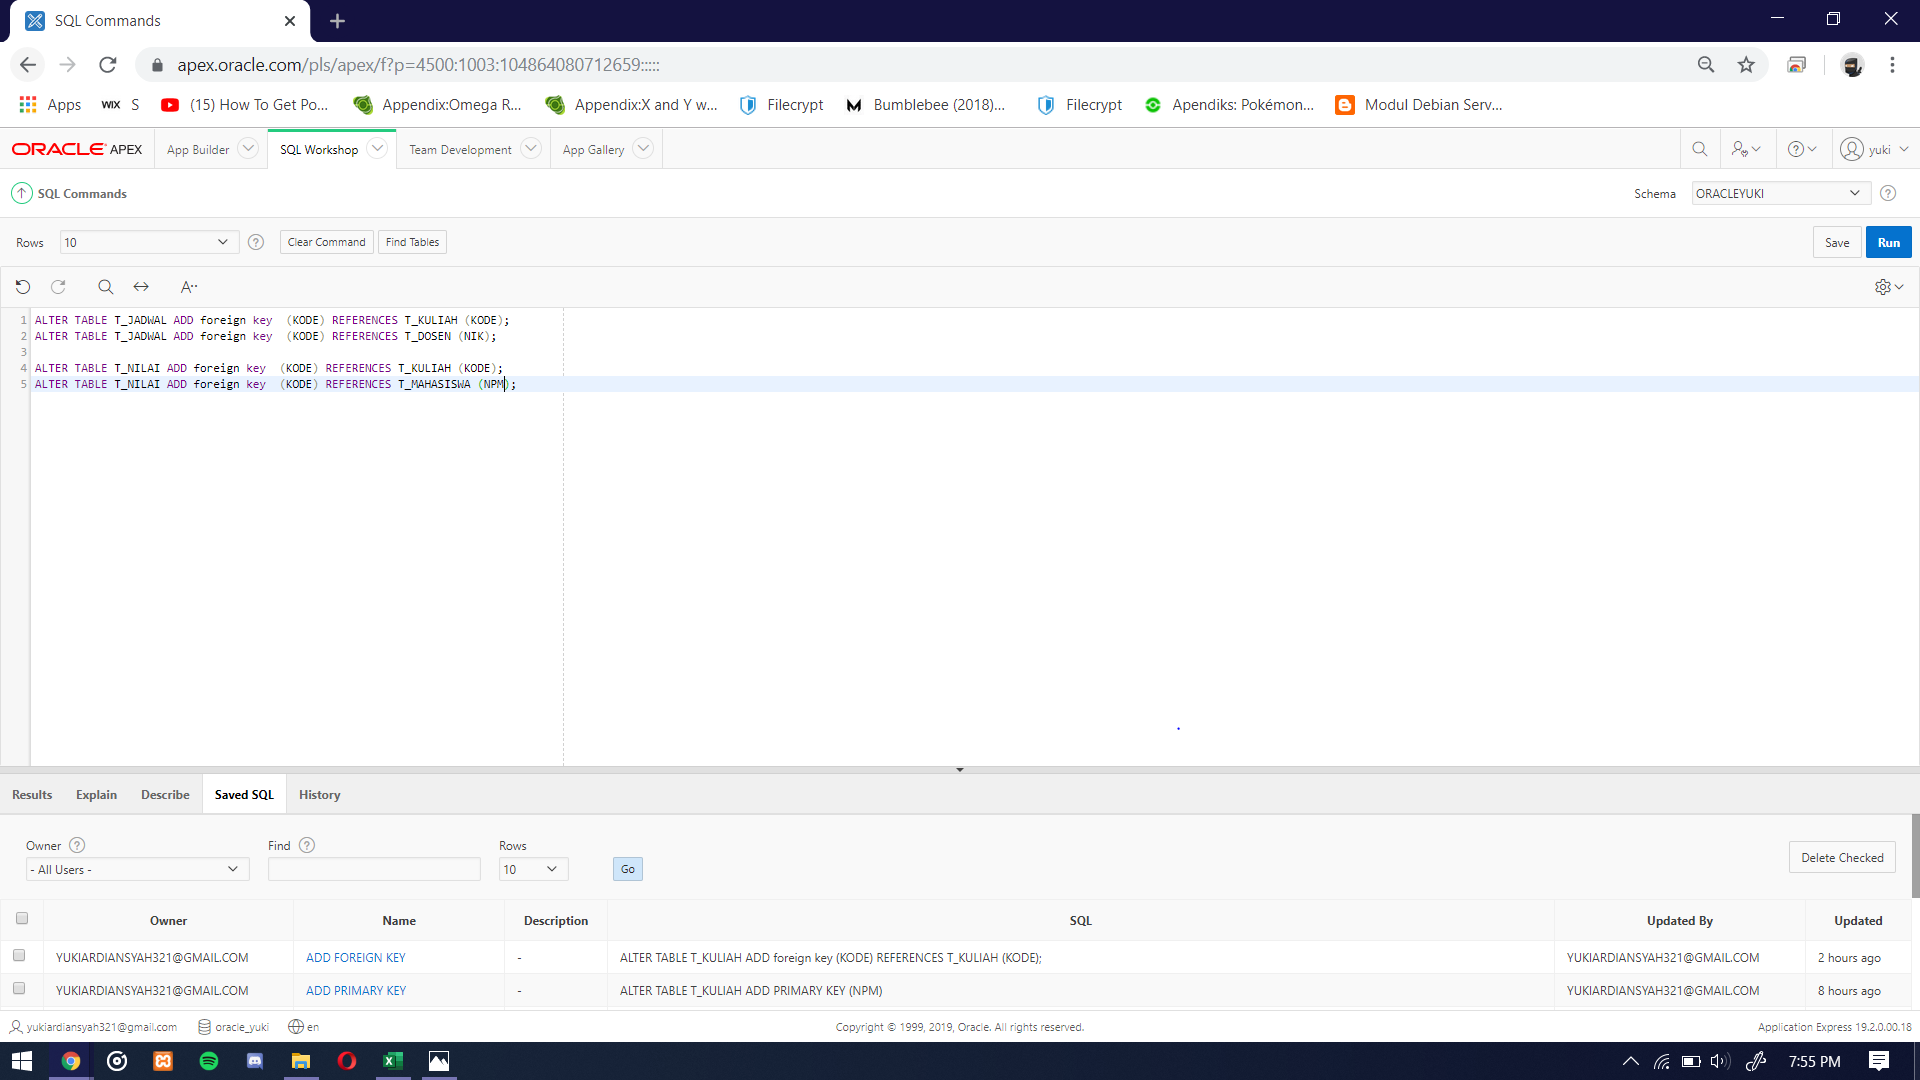
\includegraphics[scale=0.27]{figures/DB7.png}
        \caption{Membuat Foreign Key}
        \label{excel}
    \end{center}
    
      \item Setelah primary dan foreign tersetting langkah selanjutnya adalah membuat aplikasi dengan memilih pilihan ap builder-creat-new aplication
    \begin{center}
         \centering
            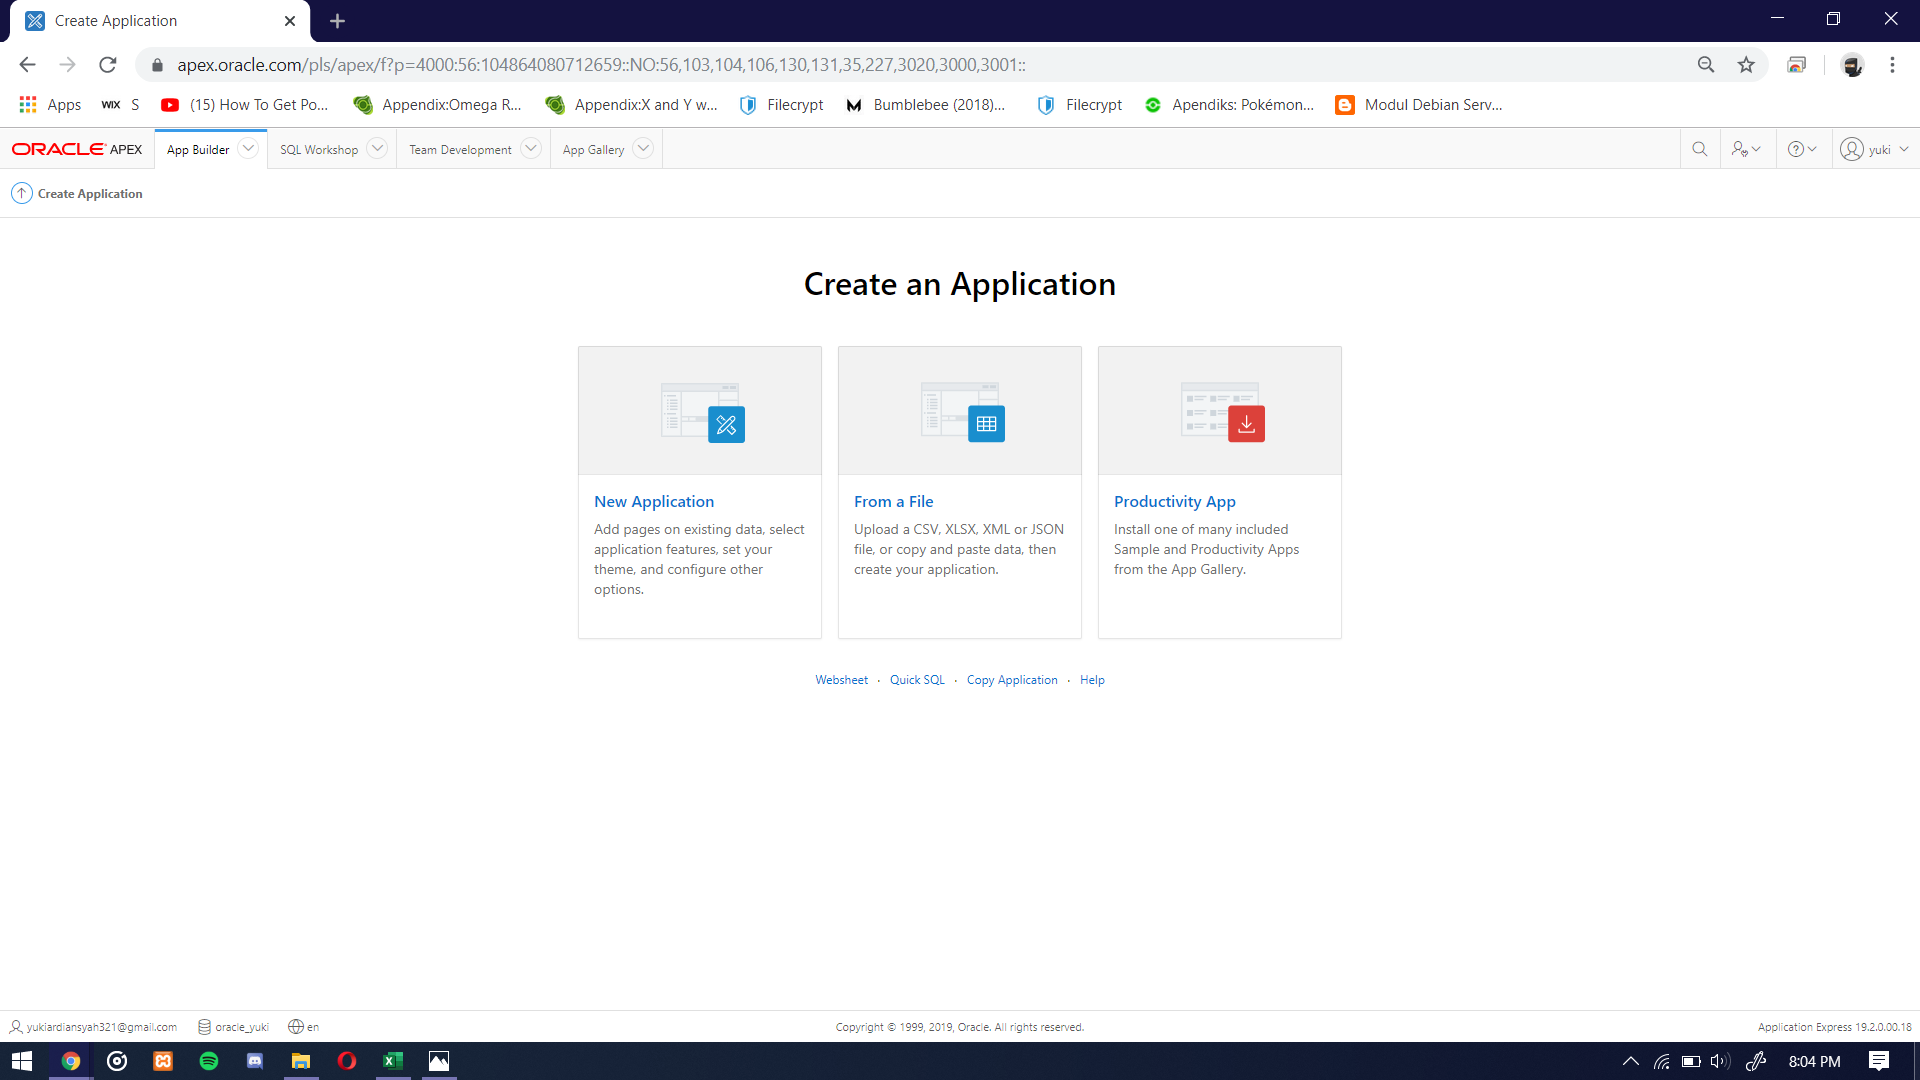
\includegraphics[scale=0.27]{figures/DB8.png}
        \caption{Tata Cara Membuat Aplikasi}
        \label{excel}
    \end{center}
    
     \item Setelah itu muncul tampilan seprti gambar dibawah pertama memberi nama dari aplication tersebut
    \begin{center}
         \centering
            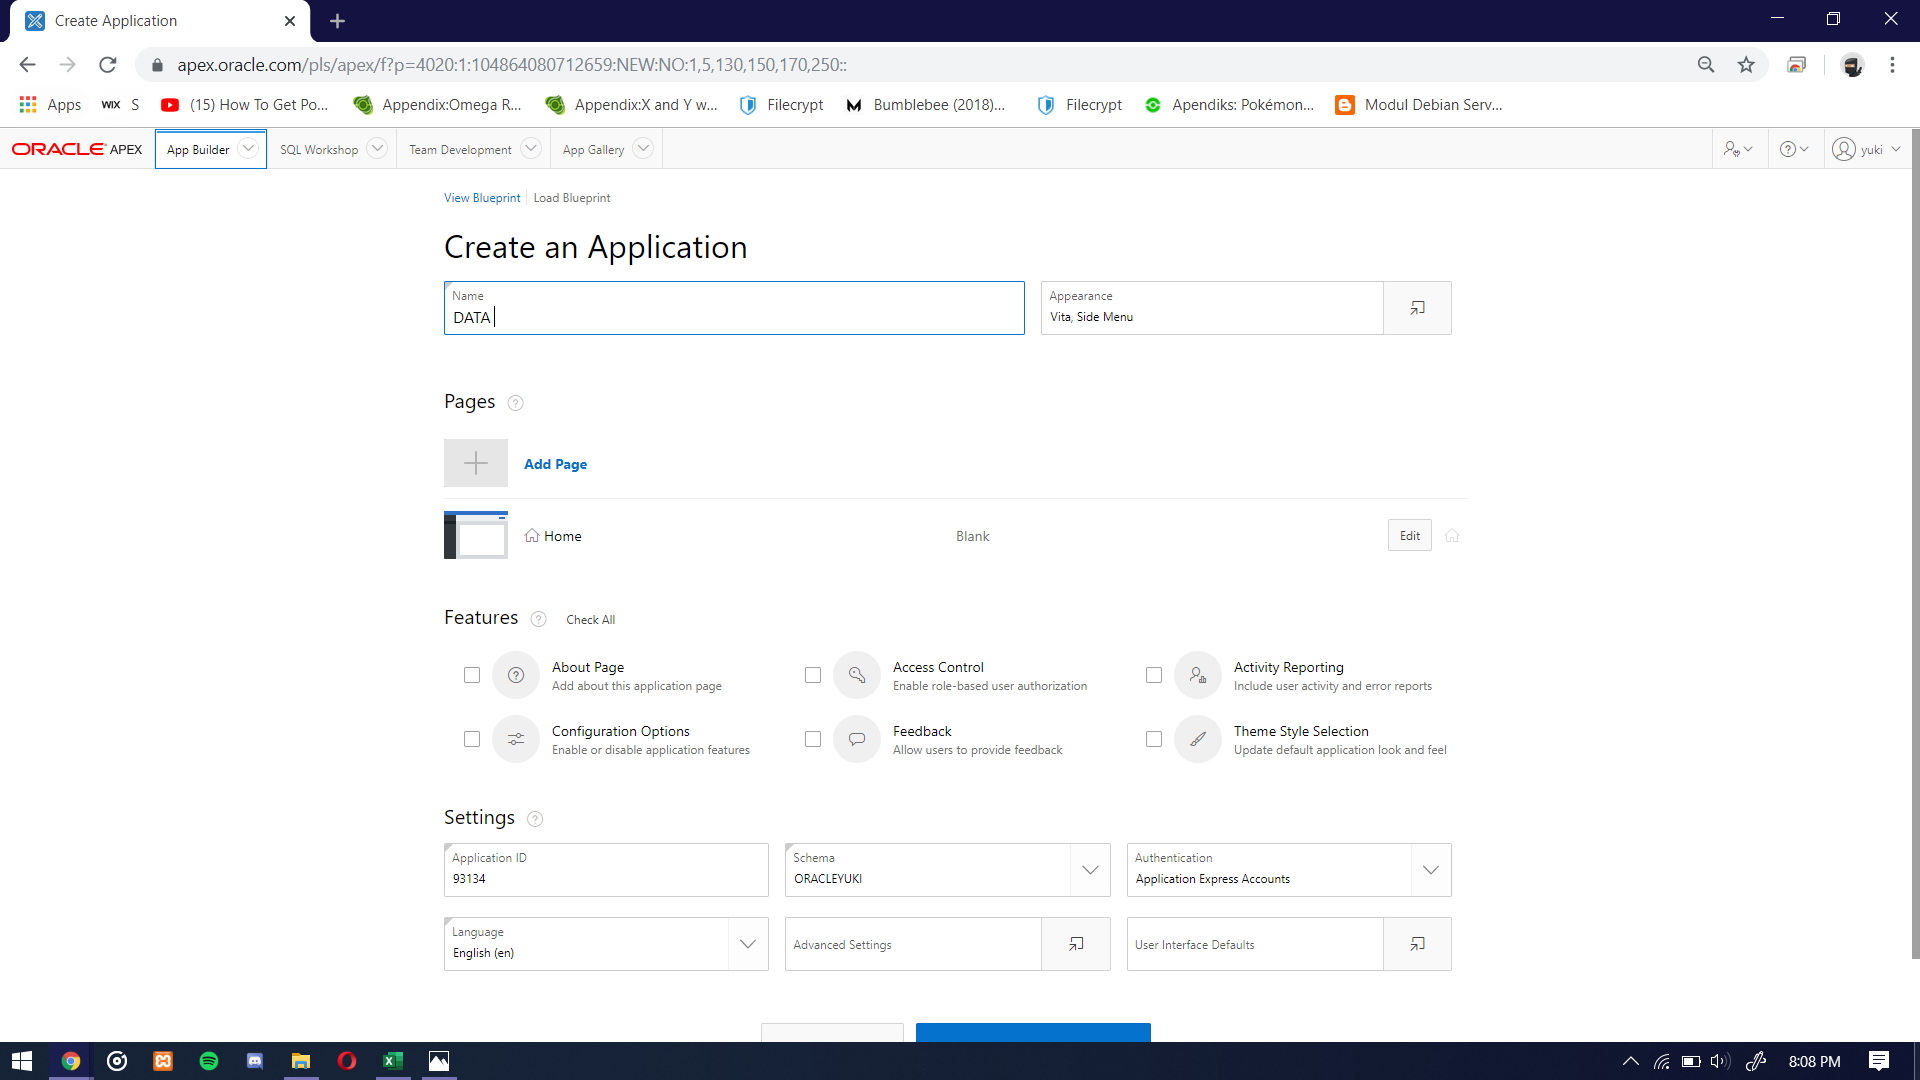
\includegraphics[scale=0.27]{figures/DB9.png}
        \caption{New Aplication}
        \label{excel}
    \end{center}
    
    \item Setelah itu Klik add page dan pilih menu interactive report
    \begin{center}
         \centering
            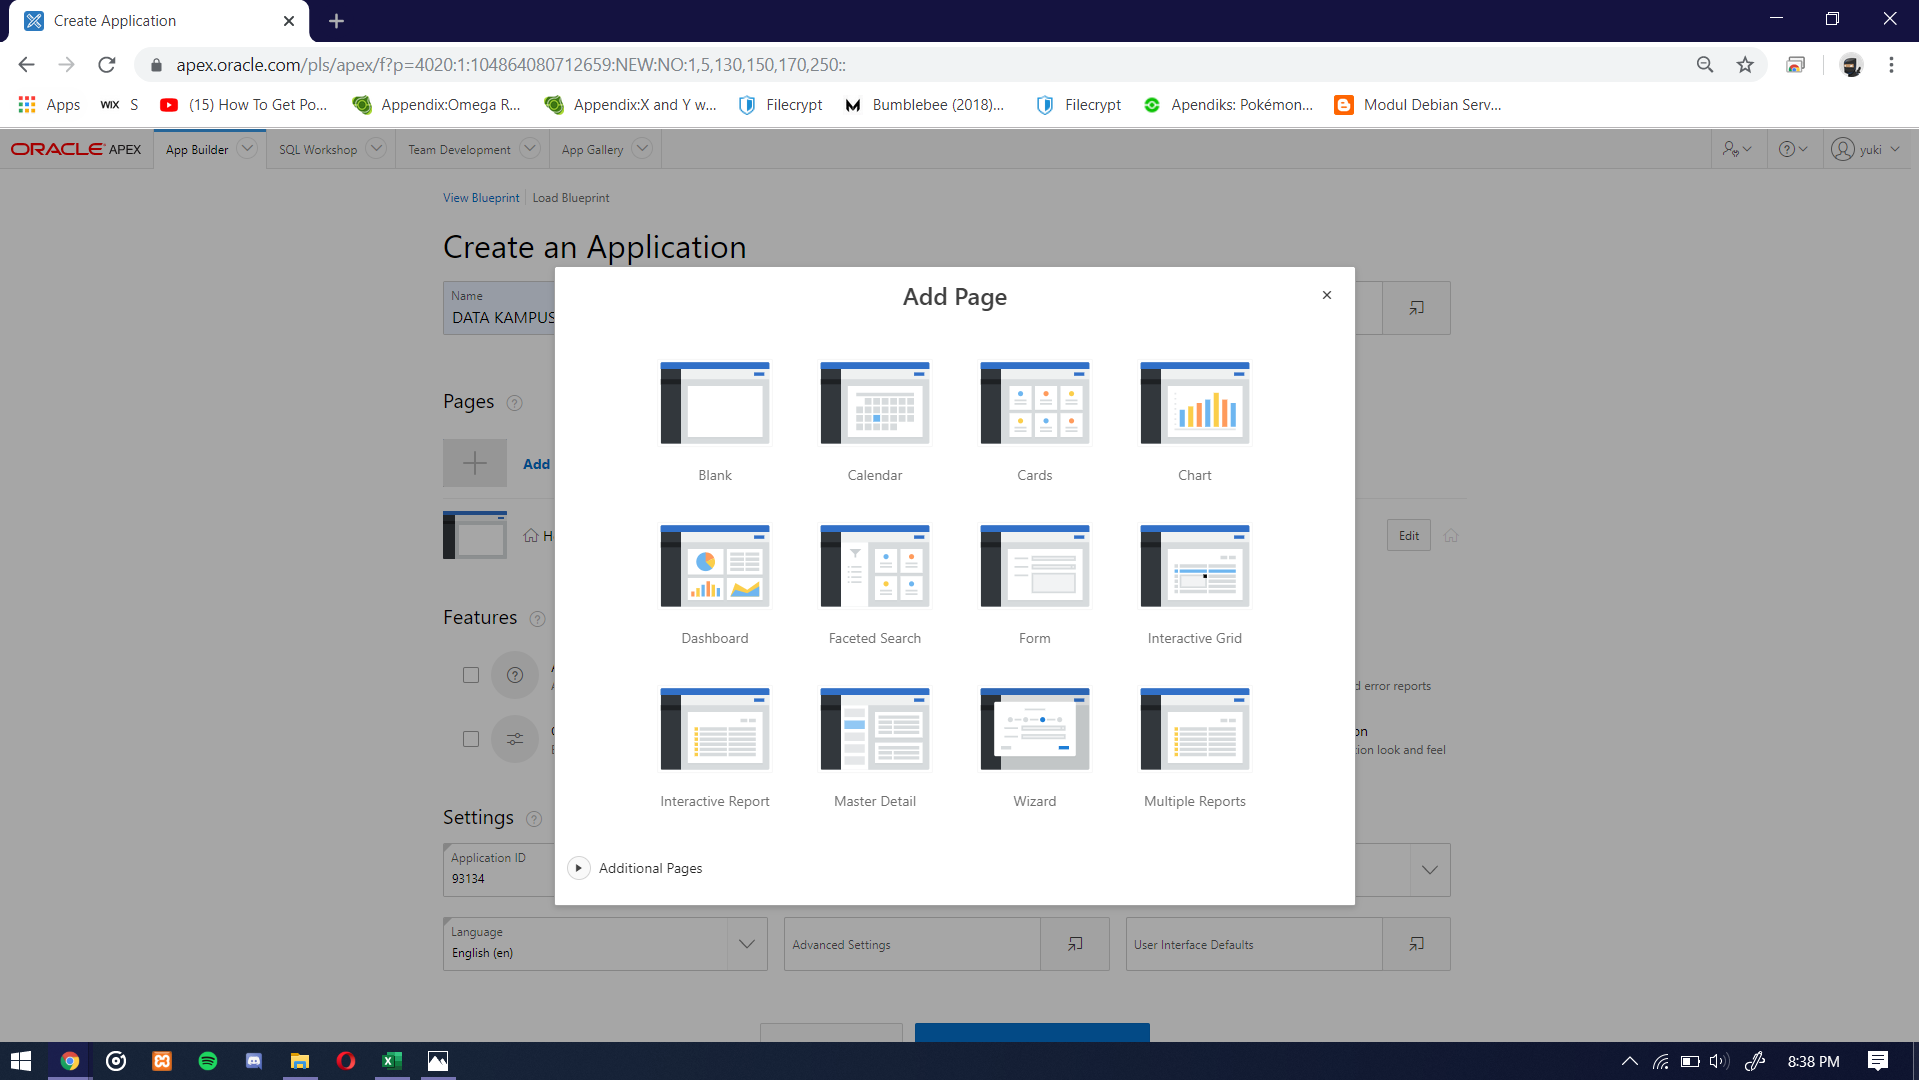
\includegraphics[scale=0.27]{figures/DB10.png}
        \caption{Klik Jenis Aplication}
        \label{excel}
    \end{center}
    
      \item setelah Add page kita menamai page name dan menambahkan table sesuai name page. lakukan hal yang sama dengan table yang lainnya
    \begin{center}
         \centering
            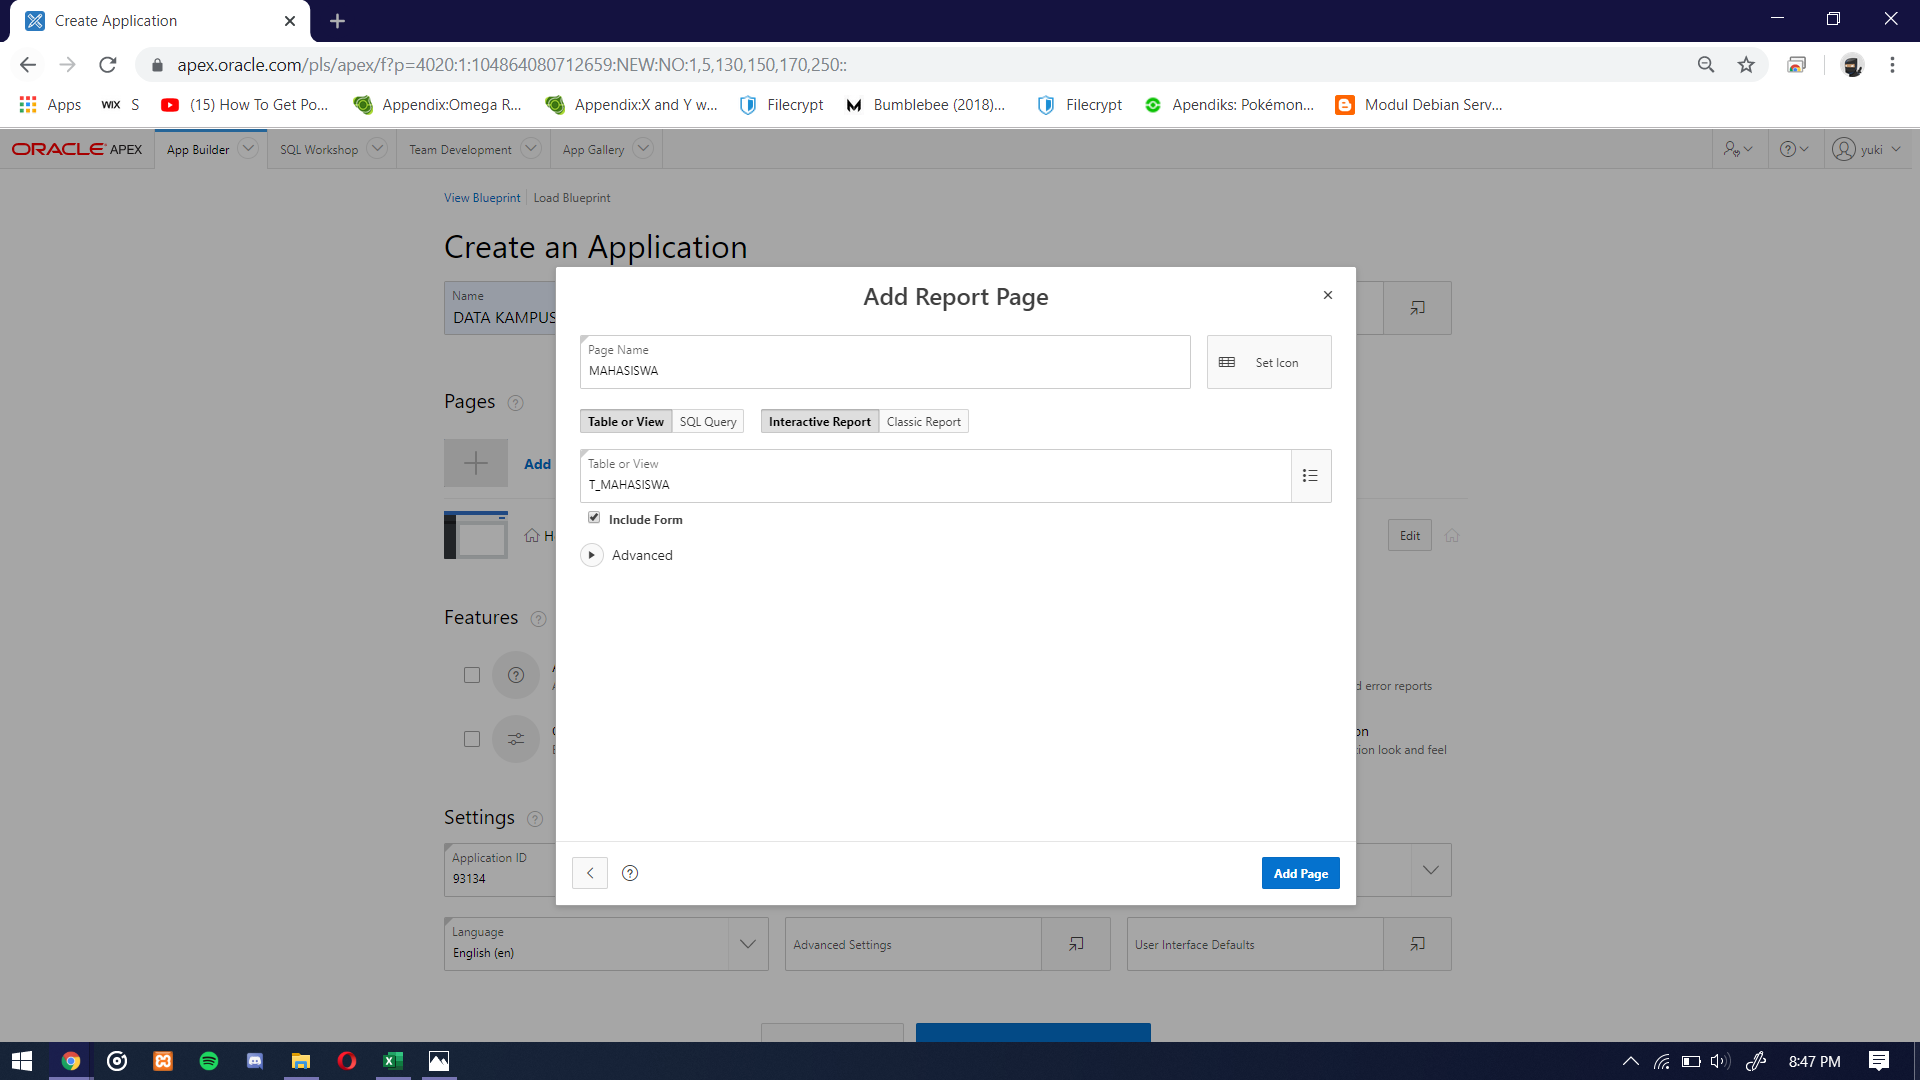
\includegraphics[scale=0.27]{figures/DB11.png}
        \caption{ADD PAGE}
        \label{excel}
    \end{center}
    
     \item Tampilan Add Page kelima table
    \begin{center}
         \centering
            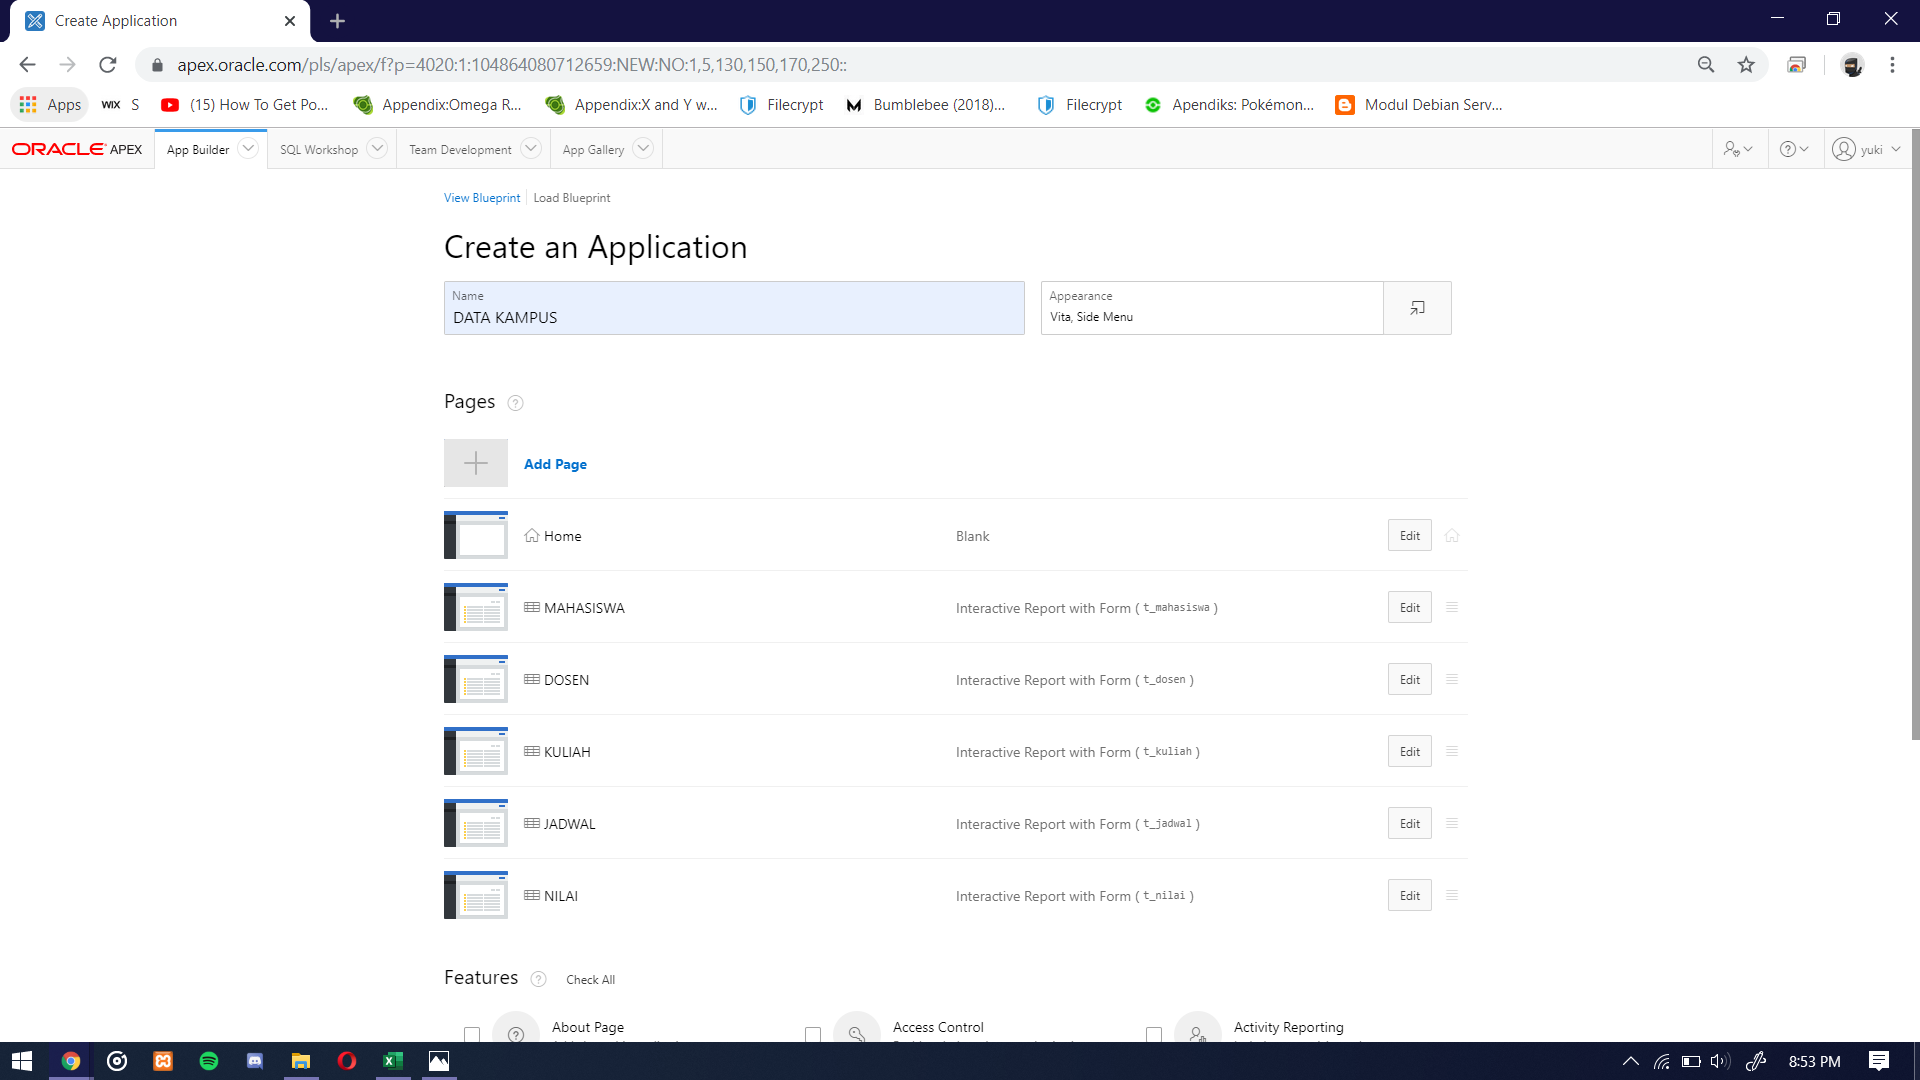
\includegraphics[scale=0.27]{figures/DB12.png}
        \caption{ADD PAGE}
        \label{excel}
    \end{center}
    
    \item Setelah Itu Run Aplications
    \begin{center}
         \centering
            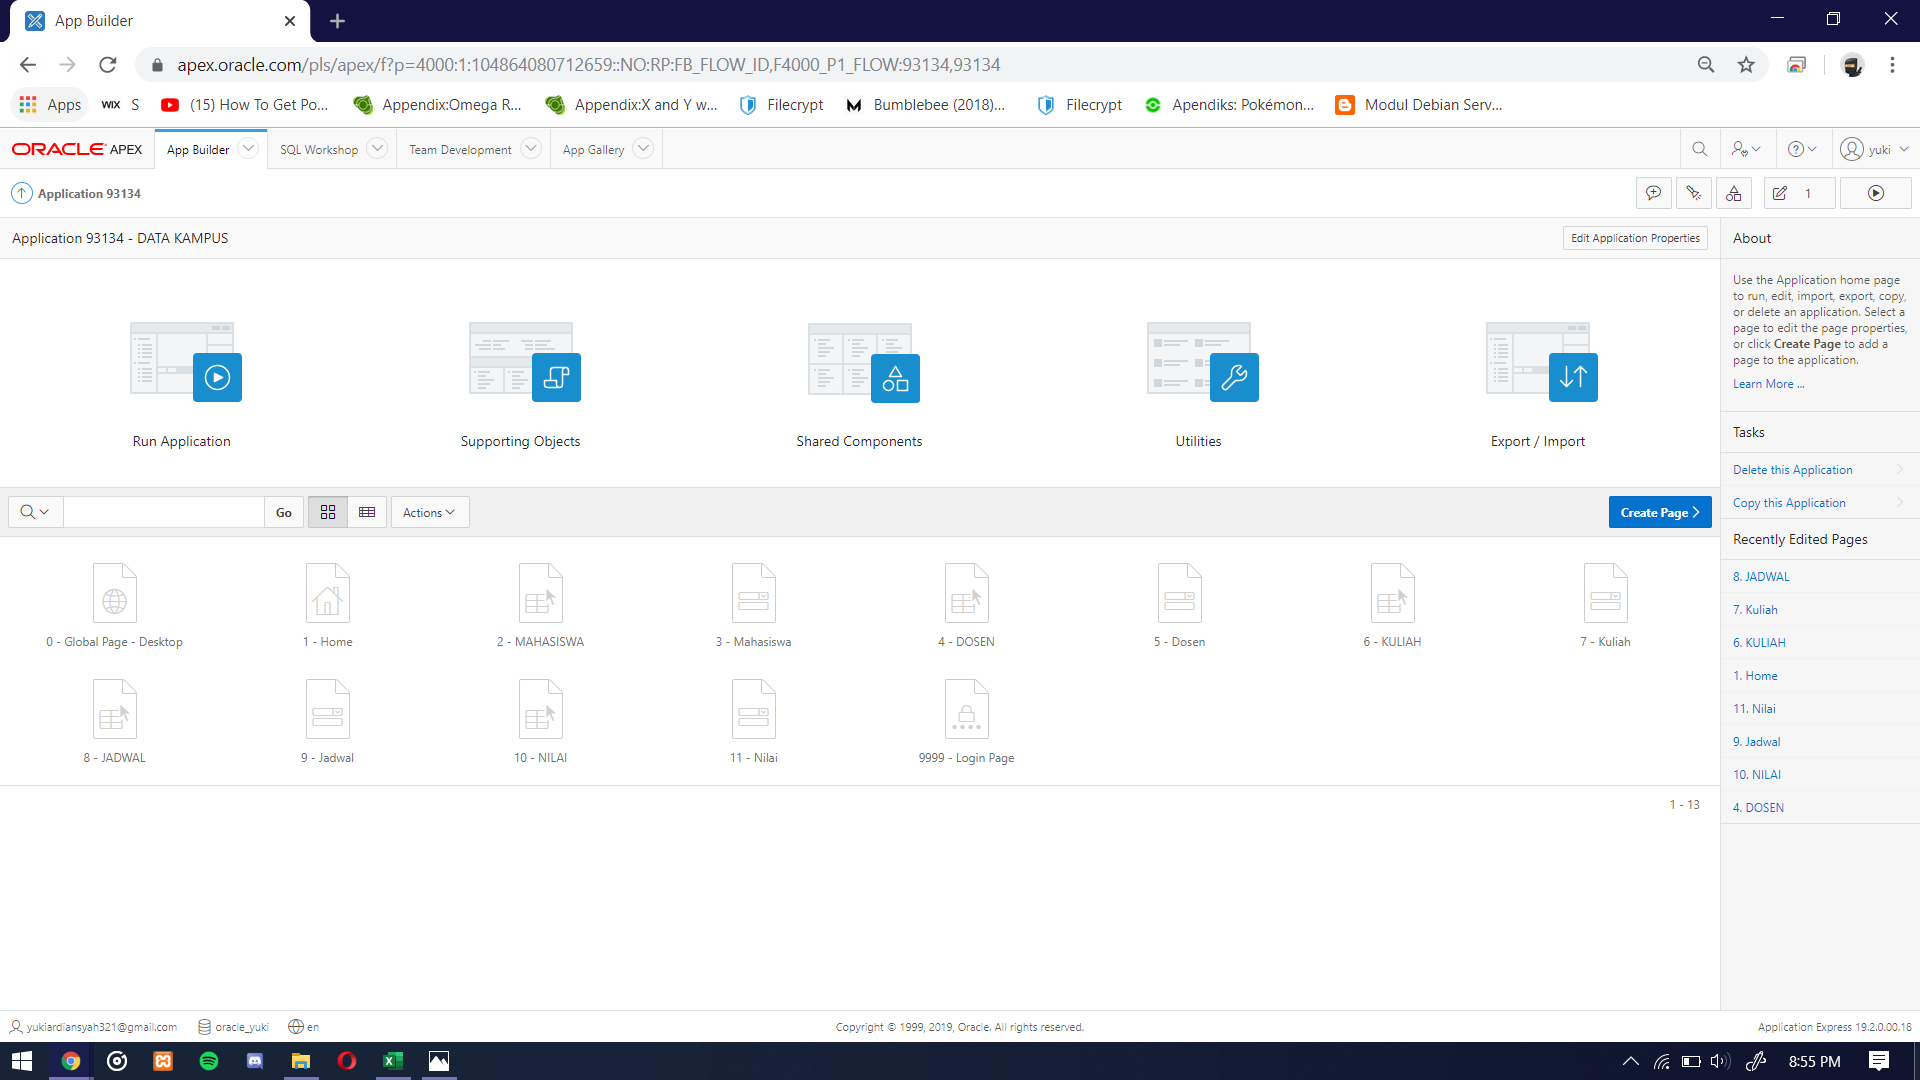
\includegraphics[scale=0.27]{figures/DB13.png}
        \caption{ADD PAGE}
        \label{excel}
    \end{center}
    
    \item Masukkan Passsword Dan Username
    \begin{center}
         \centering
            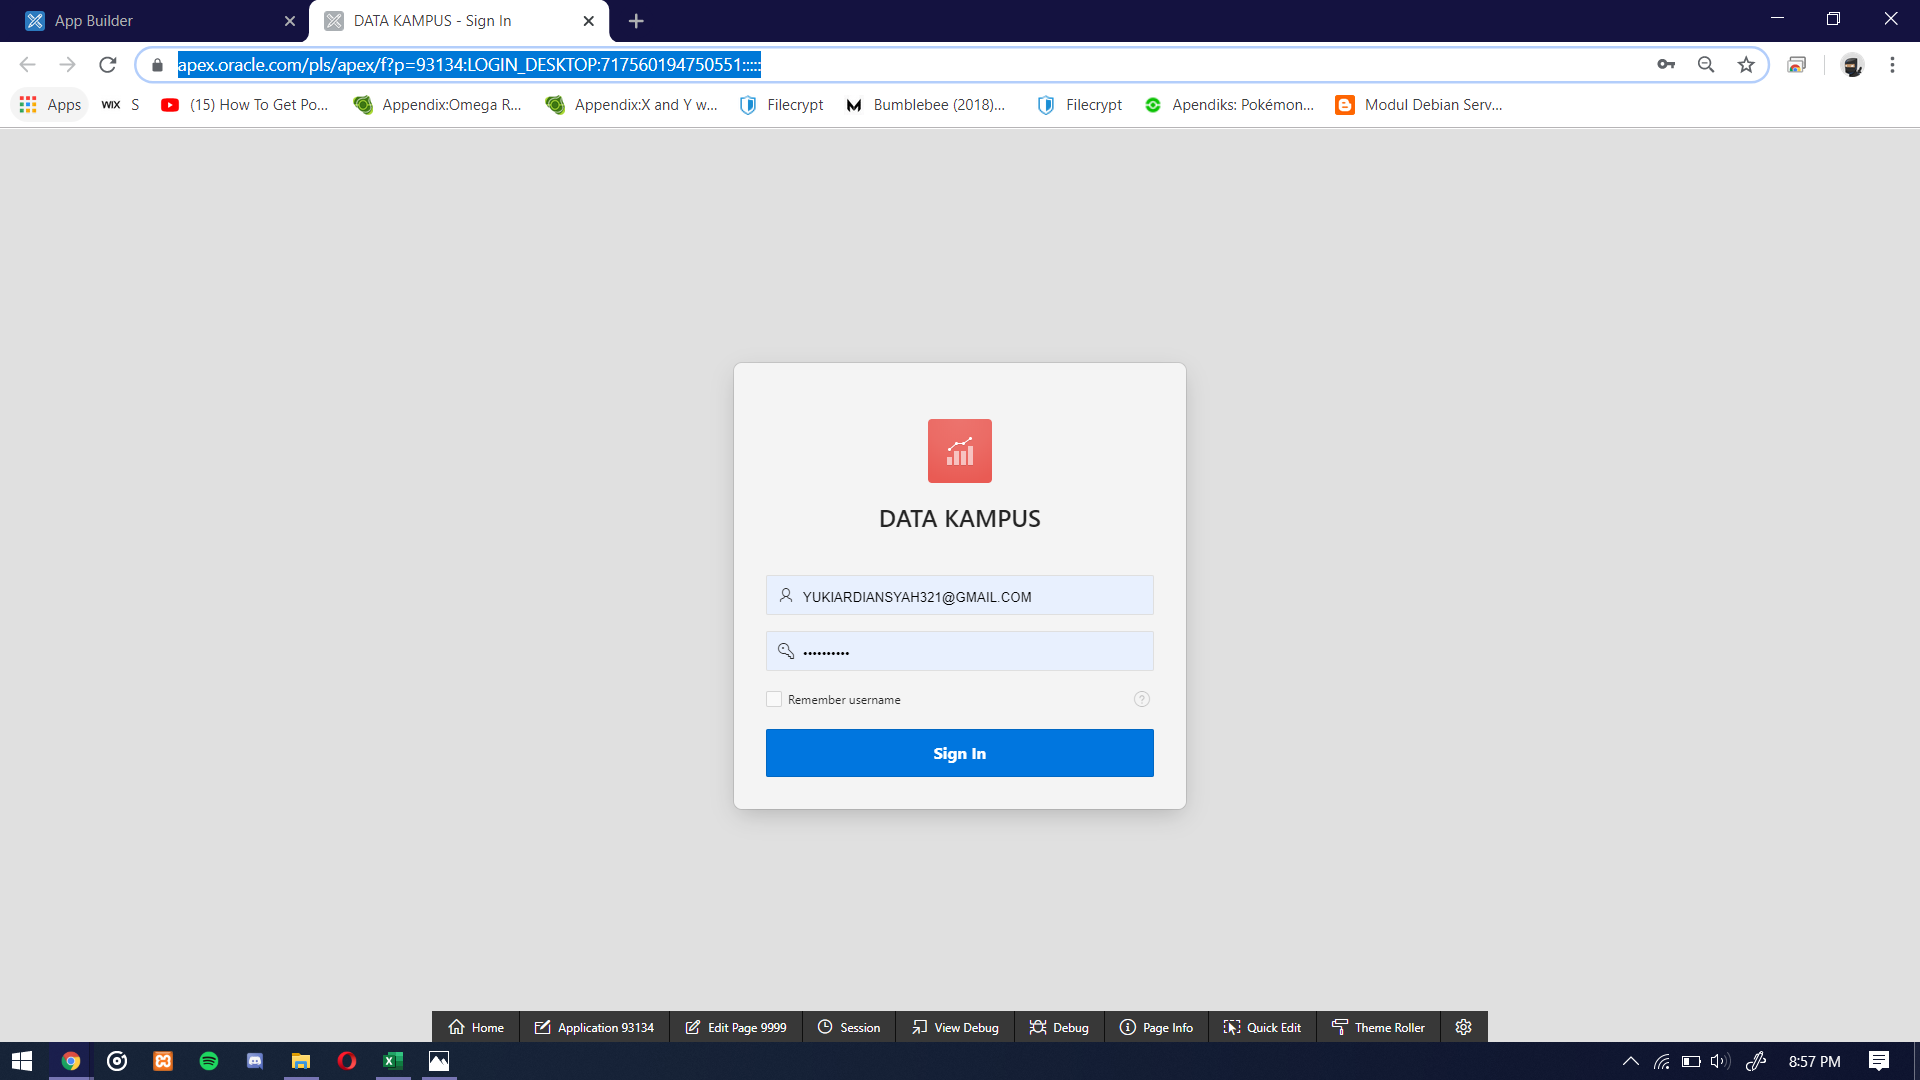
\includegraphics[scale=0.27]{figures/DB14.png}
        \caption{Masukkan Password}
        \label{excel}
    \end{center}
    
    \item Tampilan Aplikasi Yang Sudah Berjalan
    \begin{center}
         \centering
            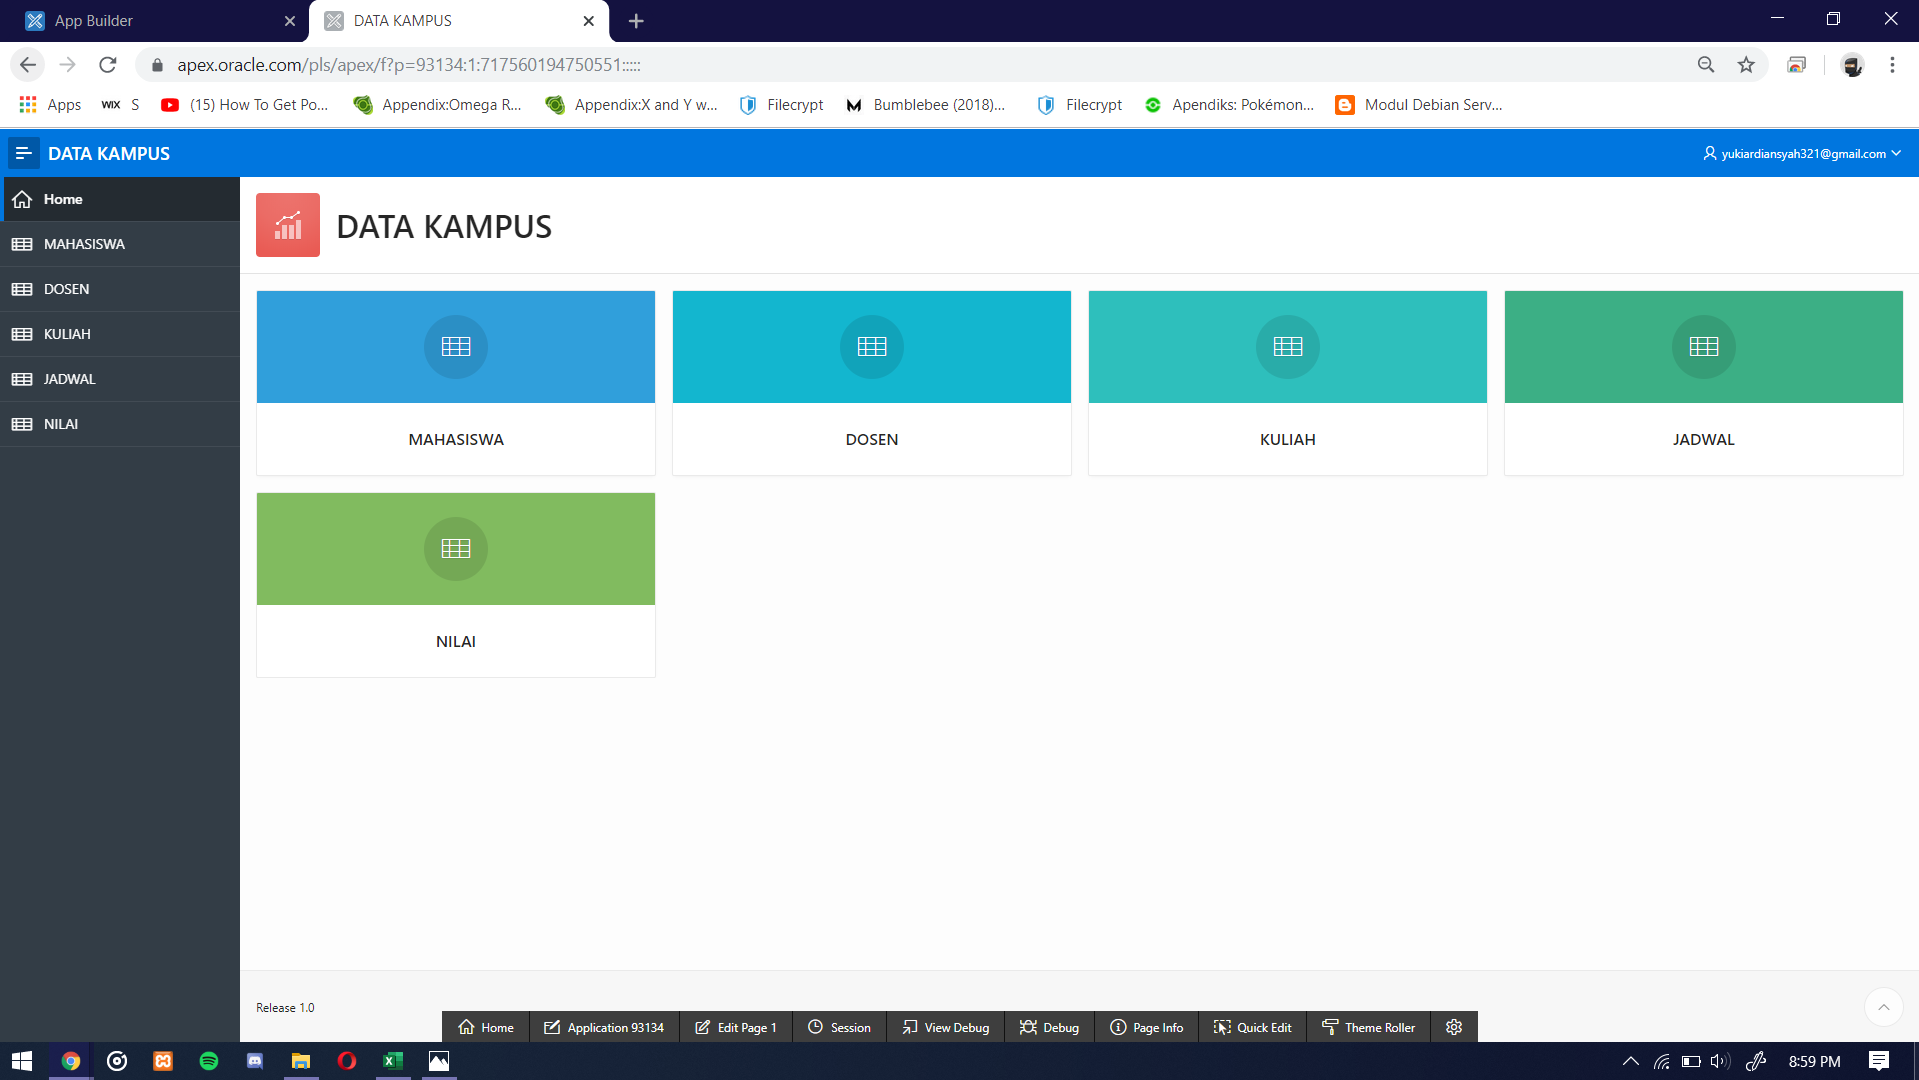
\includegraphics[scale=0.27]{figures/DB15.png}
        \caption{Masukkan Password}
        \label{excel}
    \end{center}
\end{enumerate}

\section{Password username}
      
      \begin{enumerate}
      
          \item link https://apex.oracle.com/pls/apex/f?p=93134:1:104864080712659:::::
          \item workspace "ORACLE(underscore)YUKI"
          
          \item username "YUKIARDIANSAH321@GMAIL.COM"
          
          \item password "yukiardi21"
      \end{enumerate}
      
       

\end{document}
